%%%%%%%%%%%%%%%%%%%%%%%%%%%%%
%Update: <Sep/25/2009>
%%%%%%%%%%%%%%%%%%%%%%%%%%%%%

\setcounter{chapter}{-1}
\chapter{マイクロコンピュータ応用 -導入-}
\section{はじめに}

前学期ではアセンブリプログラミングによりZ80マイコンを制御する基礎的な技術を学び
ました。本学期では, その身につけた技術を用い, スイッチ, LED, ステッピングモータなどを制御する
ことで, マイコンによる制御やプログラミングの考え方を学ぶび身につけることを目標と
します。

また, 本実験では前学期の知識を基本としているので, 前学期に用いたテキストを持参するとよ
いでしょう。

\section{レポートの書き方}

% レポートはコンピュータで作成しプリントアウトしたものを提出してください。もし図を用いる場
% 合でも画像ファイルとして, なるべく文章ファイルに挿入してください。どうしてもできないと言う場合に限
% り, 手書きの図や切り貼りでもよいです。

レポートの章立ては次のようにすると良いでしょう。

\begin{itemize}
\item 目的

      実験の目的を書く

\item 手法

      実験で用いた器具, 手法, 手順などを書く。

\item 結果

      実験内容とともに実験の結果を書く。本実験の結果では主にプログラムソースを書く。ソース
      を書く場合は, 機械語, アセンブリコード, コメントを書く。

\item 考察

考察課題や, 実験で気づいたこと, 分かったことなどを書く。

\end{itemize}

補足: レポートは, 左上の角をホッチキスでとめて下さい。


\section{マイコントレーナの使いかた}

本実験では, マイコントレーナMT-Zを用います(\figref{fig:MT-Z})。MT-Z
は8ビットマイクロプロセッサZ-80を搭載しています。レジスタには8ビットデータを記憶するこ
とができます。

\begin{figure}[htbp]
\begin{center}
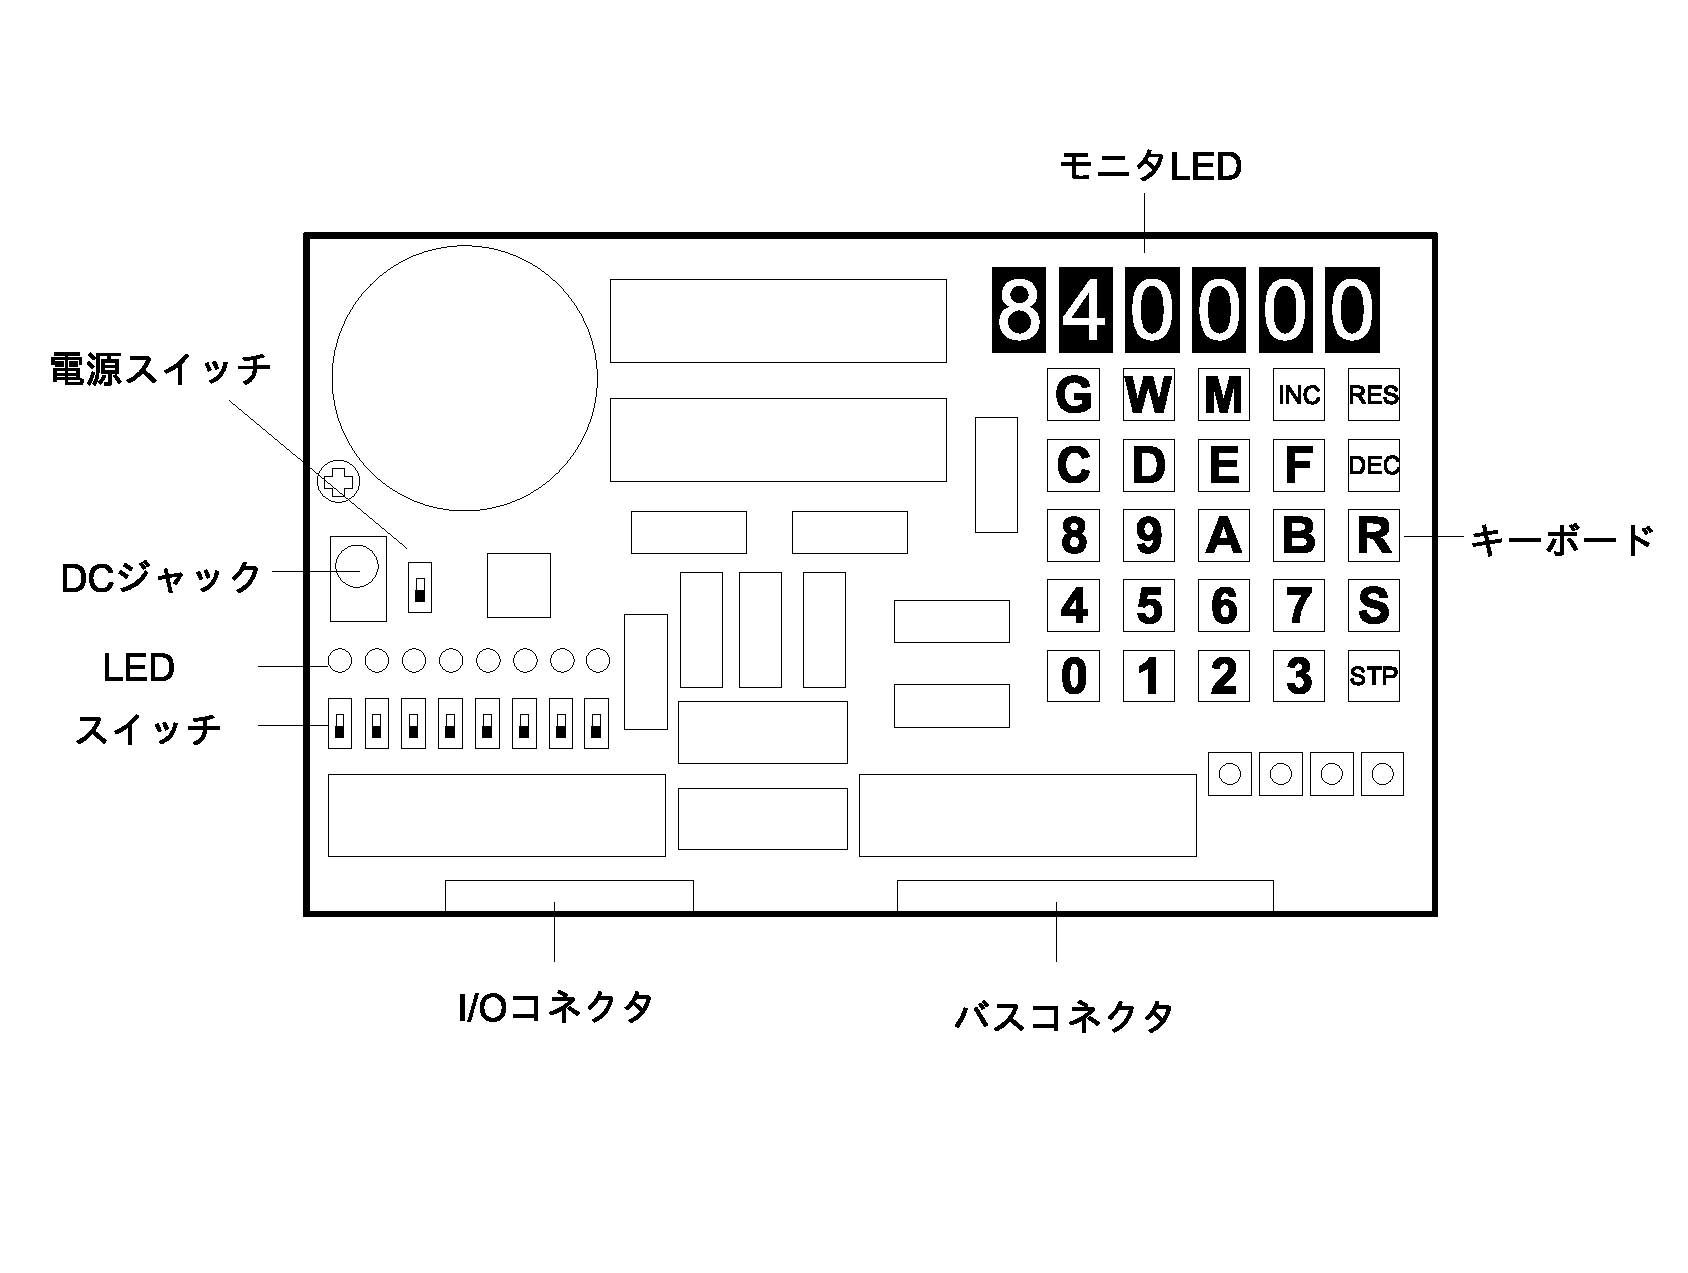
\includegraphics[width=0.8\linewidth]{img/MT-Z.eps}
\caption{マイコントレーナMT-Z。}
\label{fig:MT-Z}
\end{center}
\end{figure}

\subsection{実験開始の手順}

基本的に実験の開始は次のような手順で行います。

\begin{itemize}
\item DCジャックにACアダプタを繋ぐ。
\item ACアダプタをコンセントに繋ぐ
\item マイコントレーナの電源を入れる
\item モニタLEDが6桁とも点灯していることを確認する。
\item プログラムを入力する
\end{itemize}

\subsection{モニタLEDの見方}

メモリに書き込まれているデータを見るために, モニタLEDが存在します。
モニタLEDは6桁の16進の数を表示します。左の4桁はメモリのアドレスを表し, 右の2桁は
そのアドレスに入っているデータを表します(\figref{fig:monitor-key})。


\begin{figure}[htbp]
\begin{center}
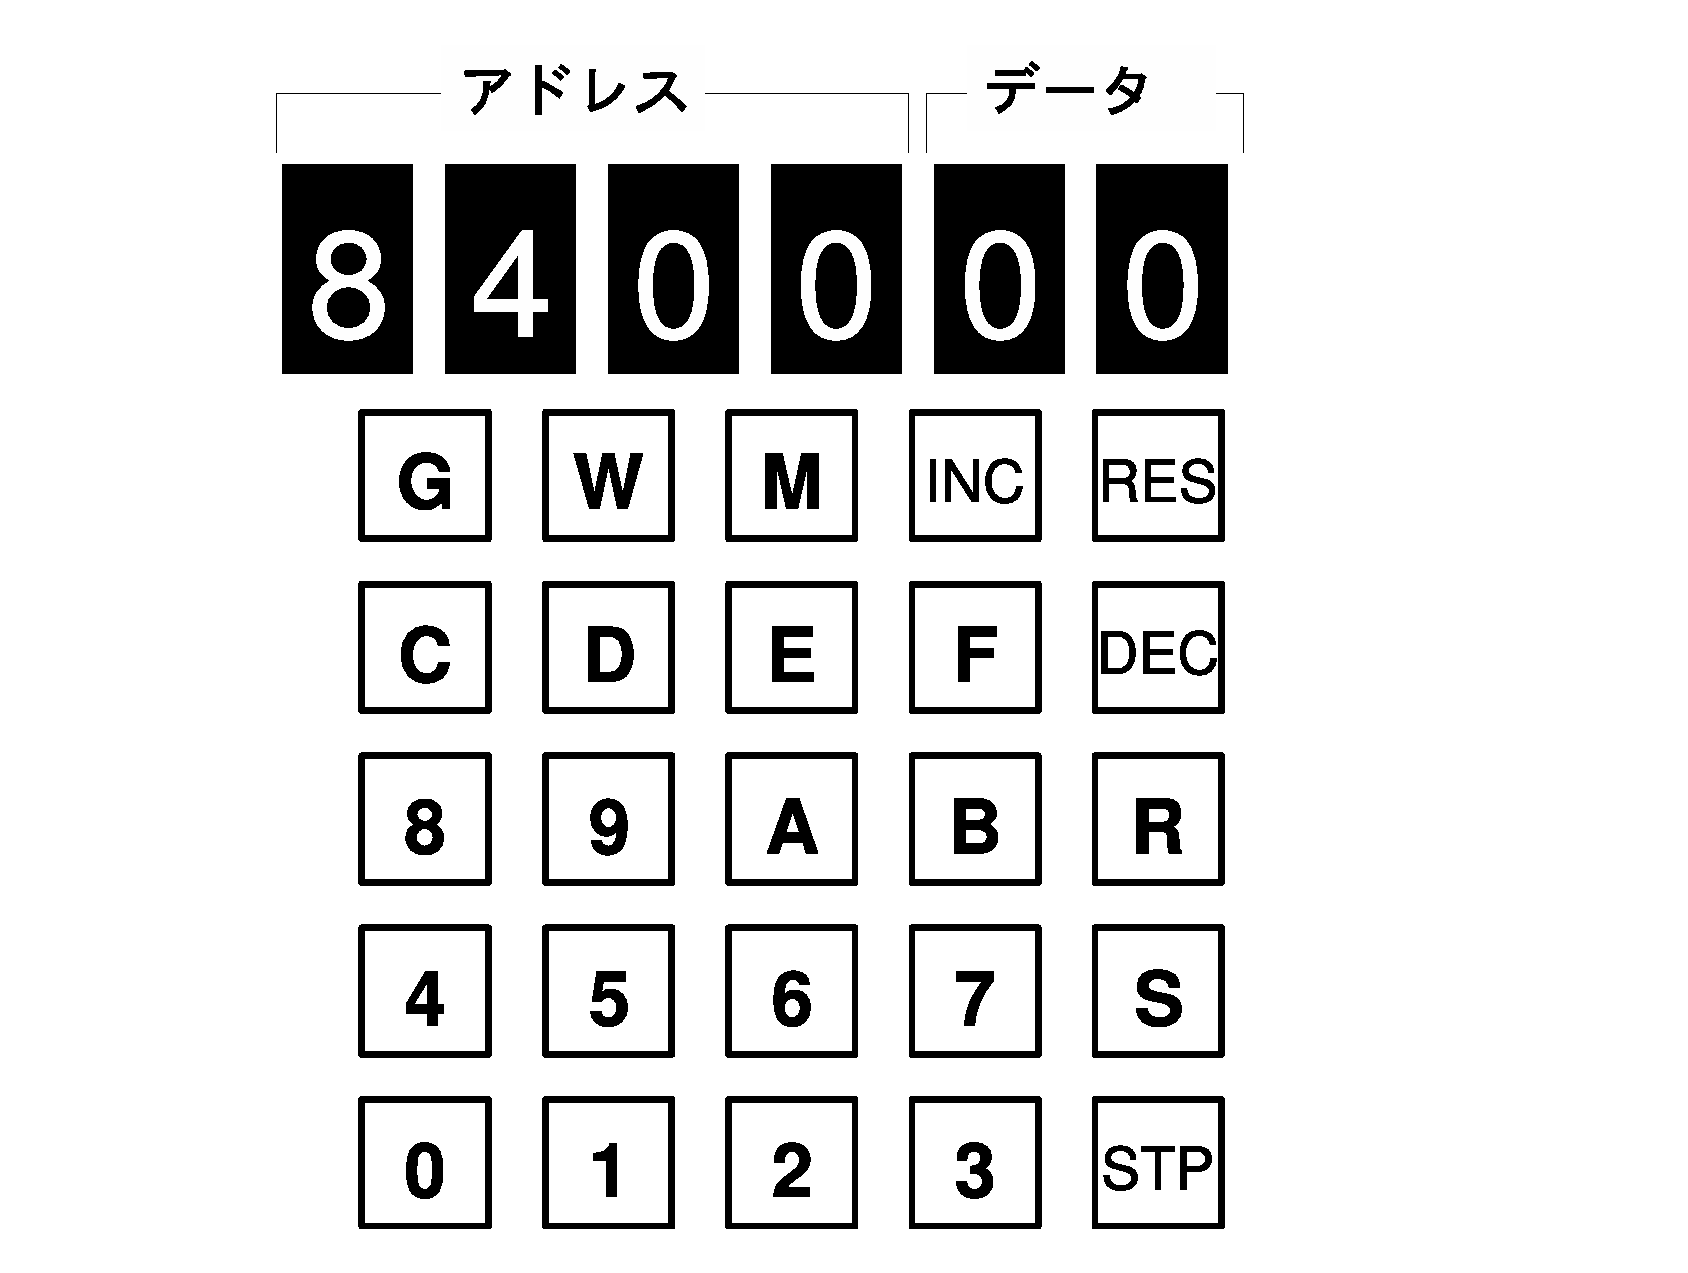
\includegraphics[width=0.5\linewidth]{img/monitor-key.eps}
\caption{モニタLED, キーボード。}
\label{fig:monitor-key}
\end{center}
\end{figure}

\subsection{メモリ内のデータの読みだしの仕方}

メモリの中に入っているデータを読み出すときにはボタンMを用います。8400H番地のデー
タを読み出すときには, Mを押して8400と入力すると8400H番地のデータが表示されます。
次の番地のデータが見たいときは, INCを押すことで次の番地に進みます。また, DECを押
すことで一つ前の番地のデータを読むことができます。

\subsection{メモリの書き込みの仕方}

メモリにデータを書き込むときは, ボタンWを用います。8400H番地に01Hというデータを
書き込む場合は, まずボタンMを押し, 8400と入力することで8400H番地に移動する。次に,
Wを押すことで書き込みモードにし,  データを入力します。次の番地に書き込みたいときには
INCを押すことで, 次の番地に書き込めます。また, DECを押
すことで一つ前の番地のデータに書き込めます。

\subsection{実験プログラムを入れることのできるメモリの領域}

実験プログラムなどを入れることができるメモリの領域は8400H--EFFFHです。実験で作っ
たプログラムはその番地に書き込んでください。サブルーティンや数値データはすぐ隣の
番地に置かず, 離れた番地に置くと, プログラムを修正する場合や書く加える時に便利で
す。

\subsection{プログラムの実行, リセットの仕方}

プログラムを実行する場合には, Gボタンを用います。8400H番地から書き込んだプログラ
ムを実行する場合は, Mボタンを押し, 次に8400と入力することで8400H番地に移動します。
そして, Gボタンを押すことでプログラムが実行されます。

もしプログラムが暴走したり, 無限ループのプログラムを終了させたいときには, RESボ
タンを押すことでプログラムを終了させることができます。

\section{本実験における作業の流れ}

本演習の多くはアセンブリプログラミング作業です。プログラミングを行う作業の流れは次の
順番で行うとよいでしょう。

\begin{itemize}
\item 処理の流れを考える。

      フローチャートなどをかいてもよい。

\item アセンブリコードを考える。

\item アセンブリコードを機械語に直す。

アセンブリコードを機械語に直すとき, テキストに付属するニーモニックと機械語の対応
      リストを参照してください。

\item 機械語をMT-Zに入力し, 実行する。
\end{itemize}

もしプログラムが動かないときは, 上記の作業の流れのうちどれかが間違っています。よ
く見直してみましょう。
